\chapter{GPU}

\begin{figure}[h]
    \centering
    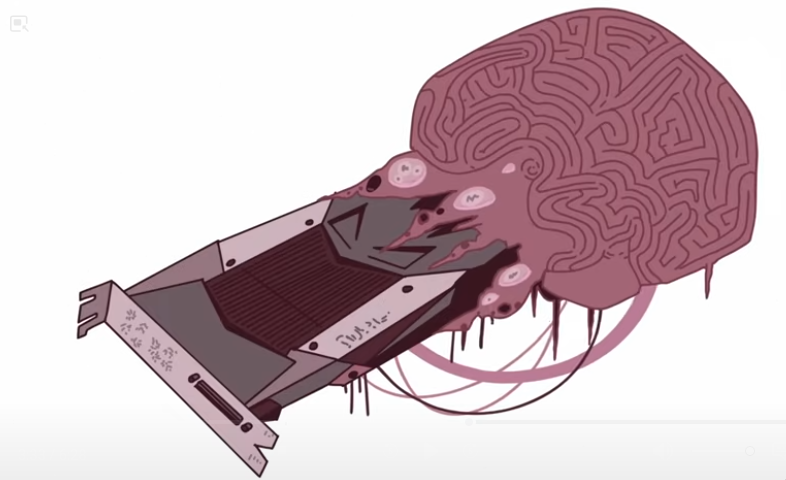
\includegraphics[scale=0.4]{06-GPU/VRAM.png}
\end{figure}

\section{Che cosa è una GPU?}

La \fancyglitter{GPU} (\textit{Graphics Processing Unit}) è un processore altamente parallelo e multithread ottimizzato per l'elaborazione visuale. Nei PC moderni viene aggiunta alla CPU per creare un sistema \fancyglitter{eterogeneo}. Benché la GPU sia il processore più potente all'interno di un normale PC, questa non può però essere da sola in quanto l'architettura che implementa l'elevato grado di parallelismo necessità di essere affiancata a una CPU che esegua al massimo delle prestazioni le operazioni sequenziali. 
A oggi le GPU non sono limitate all'elaborazione visuale, la consistente potenza di calcolo parallelo le ha rese appetibili per innumerevoli altre applicazioni (e. g. il deep learning). 
Inizialmente si effettuava il \fancyglitter{GPGPU} (\textit{General Purpouse GPU}), ovvero l'utilizzo delle API della pipeline grafica per l'elaborazione di compiti non grafici. Attualmente viene definito \fancyglitter{GPU Computing}, da quando \fancyglitter{CUDA} è stato rilasciato , in quanto si è abbandonato l'utilizzo della pipeline grafica bensì si utilizza un linguaggio di programmazione parallelo.

\dfn{CUDA}{
  CUDA (Compute Unified Device Architecture) è il modello di programmazione parallela scalabile e una piattaforma software per la GPU. Questo permette di programmare direttamente in un linguaggio simil C/C++.
}

\nt{CUDA ha un approccio SIMD (o SIMT), quindi il programmatore scrive il programma per un thread e questo viene istanziato ed eseguito da molti thread in parallelo sui molteplici processori della GPU.}

\subsection{Passaggio da GPU a CPU}

Le GPU eliminano tutto quello che è necessario per il parallelismo delle istruzioni e lasciano al programmatore la responsabilità di parallelizzare i suoi problemi (questo non è sempre possibile per cui GPU e CPU consistono in un'architettura ibrida). Inoltre sono presenti due problemi: 

\begin{itemize}
  \item \fancyglitter{Divergence Memory Wall}. 
  \item \fancyglitter{Dark Sylicon}.
\end{itemize}

\dfn{Divergence Memory Wall}{
  Negli anni le differenze di velocità tra CPU e memoria principale sono diventate troppo importanti per essere ignorate. Le GPU eliminano questo gap cercando di ridurre al minimo l'interazione con la memoria principale. 
}

\dfn{Dark Sylicon}{
  In una CPU possono stare attivi solo il 15-20\% dei transistor totali contemporaneamente, altrimenti si rischia di bruciare l'intera CPU, per questo problema vengono pensate CPU che ottengono prestazioni meno elevate ma che magari permettono un'attivazione maggiore dei transistor presenti (CPU desktop e server). Le GPU in parte permettono di ridurre anche questo problema grazie al loro alto grado di parallelismo che permette di sfruttare più transistor contemporaneamente.
}

\section{Gerarchia di Flynn}

I modelli illustrati dalla gerarchia di Flynn sono fondamentali per capire come il calcolo parallelo viene implementato in diversi contesti hardware. Ogni modello ha i suoi punti di forza e debolezza e viene utilizzato  in base alle necessità dell'applicazione.

\subsection{SISD}

\dfn{SISD (Single Instruction Single Data)}{
  Modello più semplice, solitamente utilizzato nei tradizionali processori single core. In un'architettura SISD una \newfancyglitter{singola unità di controllo} gestisce una \newfancyglitter{singola istruzione} alla volta e questa istruzione opera su un \newfancyglitter{singolo dato}.
}

\nt{
  Un normale processore di un personal computer che esegue un codice seriale. Se un programma richiede l'aggiunta di due numeri, il processore SISD eseguirà l'operazione in un singolo flusso, elaborando un'istruzione alla volta.
}

\subsection{SIMD}

\dfn{SIMD (Single Instruction Multiple Data)}{
  In un'architettura SIMD, una singola istruzione viene eseguita contemporaneamente su \newfancyglitter{molti dati}. Questo è utile per operazioni che devono essere applicate in parallelo su grandi set di dati, come il calcolo vettoriale o l'elaborazione grafica.
}

\nt{Le GPU sono un classico esempio di SIMD. Quando una GPU rendirizza un'immagine lo stesso shader (istruzione) può essere applicato a molti dati (pixel).}

\subsection{MIMD}

\dfn{MIMD (Multiple Instruction Multiple Data)}{
  In un'architettura MIMD \newfancyglitter{più istruzioni} vengono eseguite contemporaneamente su \newfancyglitter{molti dati diversi}. Questo modello è più complesso e versatile perché permette a diversi processori di eseguire diverse istruzioni su diversi dati indipendentemente. 
}

\nt{I moderni processori multicore in un computer sono esempi di MIMD. Ogni core può eseguire un thread separato, con istruzioni diverse che lavorano su dati diversi. Questo modello è utile per eseguire diversi programmi o processi simultaneamente.}

\subsection{SIMT}

\dfn{SIMT (Single Instruction Multiple Thread)}{
  È un modello ibrido che combina aspetti di SIMD e MIMD. Utilizzato prevalentemente nelle GPU moderne, consente a \newfancyglitter{molti thread} di eseguire istruzioni su dati diversi. Tuttavia, a differenza del SIMD puro, i thread in un blocco SIMT possono divergere\footnote{Prendere percorsi diversi nel flusso di controllo del programma.}.
}

\nt{
  Le GPU NVIDIA utilizzano il modello SIMT. Ogni \fancyglitter{WARP}\footnote{Gruppo di thread.} in una GPU NVIDIA esegue la stessa istruzione, ma su dati diversi. Se alcuni thread di un WARP devono eseguire un'istruzione condizionale (e. g. IF), possono divergere e successivamente riconvergere, ma sono ancora coordinati dal modello SIMT.  

}

\section{Elaboratori Moderni}

\subsection{Schema Generale}

L'architettura di un sistema di calcolo eterogeneo composto da CPU e GPU può essere descritta ad alto livello prendendo in considerazione due caratteristiche principali: 
\begin{itemize}
  \item Il numero di sottosistemi funzionali. 
  \item Il tipo di tecnologia di interconnessione.
\end{itemize}

\begin{figure}[h]
    \centering
    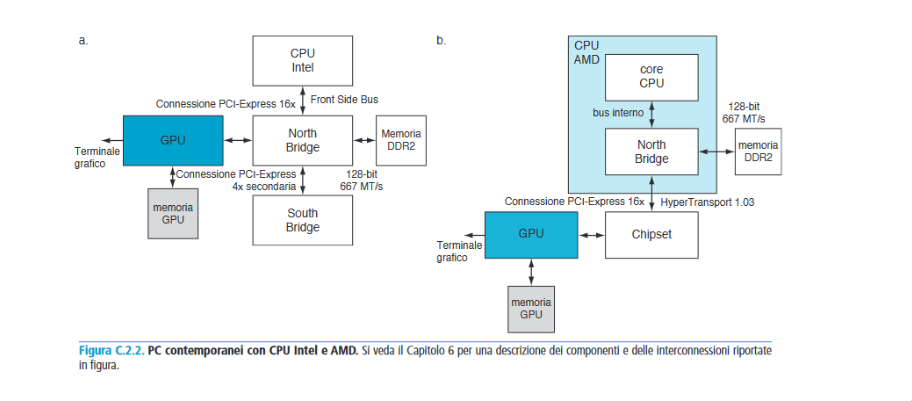
\includegraphics[scale=0.5]{06-GPU/Mod_arch.png}
    \caption{Schema di un elaboratore moderno.}
\end{figure}

\nt{Il \fancyglitter{north bridge} contiene le interfacce a banda larga che connettono la CPU, la memoria e il PCI.}

\subsubsection{}

Nella figura a è riportato lo schema INTEL dove la GPU è connessa mediante un collegamento \fancyglitter{PCI-EXPRESS} 2.0 a 16 vie che fornisce una velocità di trasferimento di picco di 16 GB/s (8 in ogni direzione). Nella figura b è riportato lo schema AMD nel quale la GPU è connessa al chipset, anche in questo caso tramite PCI-EXPRESS. In entrambi i casi GPU e CPU possono accedere alla memoria l'una dell'altra, seppure con una larghezza di banda minore che nel caso di accesso diretto. 

Le GPU possono accedere alla propria memoria locale e alla memoria fisica di sistema della CPU utilizzando indirizzi virtuali che vengono tradotti da un'unità di calcolo dedicata di gestione della memoria (MMU, Memory Management Unit) a bordo della GPU. Sarà il kernel del sistema operativo a gestire la tabella delle pagine della GPU: si può accedere a una pagina fisica della memoria di sistema mediante transazioni sulla connessione PCI-EXPRESS coerenti o non-coerenti, a seconda del valore di un attributo specificato nella tabella delle pagine della GPU. La CPU può accedere alla memoria locale della GPU attraverso un intervallo di indirizzi nello spazio di indirizzamento del bus PCI-EXPRESS.

\subsection{Architettura di una GPU}

Le architetture di GPU unificate sono basate su una schiera di molti processori programmabili che unificano l'elaborazione effettuata dagli shader dei vertici, della geometria e dei pixel e il calcolo generico sugli stessi processi, a differenza delle GPU precedenti che avevano processori separati dedicati a ciascun tipo di elaborazione. L'insieme dei processori programmabili è strettamente integrato con alcuni processori che hanno una funzione prefissata, come il filtraggio della tessitura, la rasterizzazione, le operazioni sulla memoria video, l'anti-aliasing, la compressione, la decomposizione, la visualizzazione, la decodifica video e l'elaborazione video ad alta definizione. 

Rispetto alle CPU multicore, le GPU a più core presentano una differente filosofia di progetto dell'architettura, che è focalizzata sull'esecuzione di molti thread paralleli su più processori in modo efficiente. Utilizzando molti core più semplici e ottimizzando il parallelismo sui dati tra gruppi di thread, una frazione maggiore di transistor per ogni chip è dedicata all'elaborazione e non alla memoria cache interna o funzioni accessorie.

\begin{figure}[h]
    \centering
    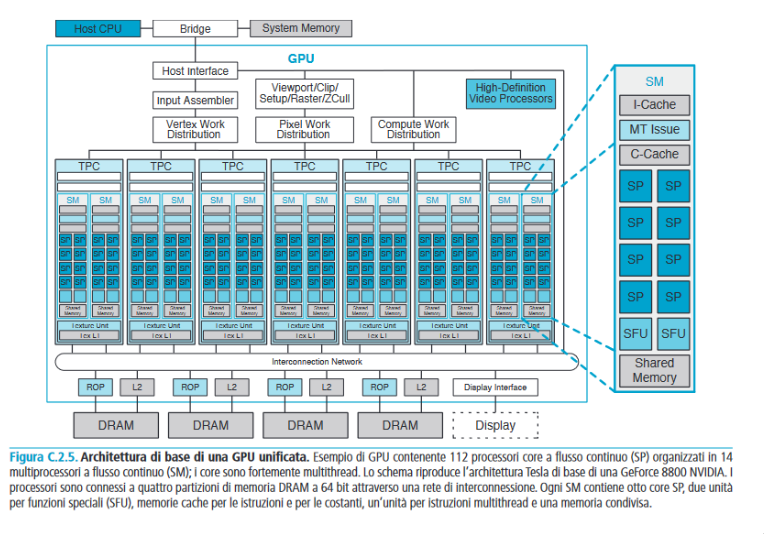
\includegraphics[scale=0.5]{06-GPU/GPU.png}
    \caption{Architettura di una GPU.}
    \label{fig:GPU}
\end{figure}

Una schiera di processori unificati di una GPU contiene molti processori core, tipicamente organizzati in multiprocessori multithread. In figura \ref{fig:GPU} è mostrata una GPU contente un'insieme di 112 processori core a flusso continuo (SP, Streaming Processor) organizzati in 14 multiprocessori multithread a flusso continuo (SM, Streaming Multiprocessor). Ogni core SP è altamente multithread, essendo in grado di gestire in hardware 96 thread concorrenti e il loro stato. I processori sono connessi a 4 partizioni di memoria DRAM a 64 bit attraverso una rete di interconnessione. Ogni SM  contiene 8 core SP, 2 unità per funzioni speciali (SFU), memorie cache per le istruzioni e le costanti, un'unità per le istruzioni multithread e una memoria condivisa. Questa è l'architettura di base implementata nella scheda \fancyglitter{GeForce 8800 di NVIDIA}.

L'architettura a schiera di processori consente di creare configurazioni di GPU, modificando il numero dei multiprocessori e il numero di partizioni di memoria. Il numero dei processori e il numero delle memorie può variare, al fine di progettare sistemi basati su GPU che siano bilanciati per differenti prestazioni e destinati a differenti segmenti di mercato.

Il sottosistema di memoria è il componente principale per le prestazioni del sistema grafico. I sistemi di memoria delle GPU devono possedere le seguenti caratteristiche:

\begin{itemize}
  \item \fancyglitter{Ampiezza Elevata:} è presente un elevato numero di piedini per trasferire i dati tra  la GPU e i suoi dispositivi di memoria e che la struttura a matrice della memoria stessa è composta da molti chip di DRAM in modo da poter sfruttare tutta la larghezza del bus dati. 
  \item \fancyglitter{Elevata velocità:} sono implementate tecniche aggressive di segnalazione per massimizzare la velocità di trasferimento dei dati (bit/s) per ogni piedino del chip.
  \item Le GPU cercano di utilizzare ogni ciclo di clock disponibile per trasferire dati da o verso la matrice della memoria. Per raggiungere questo obiettivo nelle GPU non si cerca di minimizzare la latenza del sistema di memoria: un throughput elevato (efficienza di utilizzo) e una latenza bassa sono intrinsecamente in conflitto. 
  \item Vengono impiegate tecniche di compressione, sia con perdita di informazione (eventualità di cui il programmatore deve essere ben consapevole) sia senza perdita, le quali vengono applicate in maniera opportunistica e risultano trasparenti alle altre applicazioni. 
  \item Cache e strutture che fondono le richieste di trasferimento vengono utilizzate per ridurre la quantità di traffico richiesto fuori dal chip e per garantire che i cicli di clock spesi per il trasferimento dei dati vengano sfruttati nella maniera più completa possibile.
\end{itemize}

\qs{}{Ma come viene gestita la memoria?}

\begin{itemize}
  \item \fancyglitter{Memoria Globale:} risiede nella DRAM esterna e non è locale a nessuno degli SM, poiché è pensata per la comunicazione tra i diversi CTA (blocchi di thread) di griglie diverse. 
  \item \fancyglitter{Memoria Condivisa:} è dedicata a ciascun CTA, è visibile soltanto ai thread che appartengono a quel CTA e alloca spazio di memoria solo dall'istante in cui il CTA viene creato fino all'istante in cui termina. Per questi motivi spesso risiede sul chip del SM per limitare al minimo i tempi di interazione. 
  \item \fancyglitter{Memoria Locale:} questa è dedicata a ciascun thread, è una memoria privata visibile soltanto al singolo thread. Dal punto di vista architetturale è più grande dell'insieme dei registri di thread. Per permettere di allocare vaste aree di memoria si usa la DRAM esterna.
\end{itemize} 

\nt{La memoria globale e locale, essendo che risiedono esternamente al chip, si prestano ad avere la propria cache nel chip.}

\section{Programmare una GPU: CUDA}

La programmazione di una GPU differisce in maniera sostanziale dalla programmazione degli altri multiprocessori. I modelli di programmazione delle GPU e i programmi applicativi vengono progettati per coprire una vasta gamma di gradi di parallelismo. Il motivo per cui è necessario disporre di molti core ed eseguire svariati thread in parallelo è rappresentato dalla grafica in tempo reale (solo un sistema di questo tipo permette il rendering di scene 3D complesse ad alta risoluzione). Analogamente il modello di programmazione CUDA permette a generiche applicazioni di calcolo parallelo di sfruttare grandi quantità di thread paralleli e funzionare su un numero qualsiasi di processore core in modo trasparente all'applicazione. Il programmatore scrive il codice per un singolo thread, ma la GPU lancia un numero elevato di istanze del thread in parallelo. 

\subsection{Decomposizione di un Problema}

Per mappare in modo efficace problemi di calcolo di grandi dimensioni su un'architettura altamente parallela, il programmatore o il compilatore devono scomporre il problema in tanti problemi più piccoli che possono essere risolti in parallelo. Per esempio: il programmatore può partizionare un grande vettore di dati contente il risultato in blocchi e poi partizionare ulteriolmente ogni blocco in elementi più piccoli, così che i blocchi del risultato possano essere determinati indipendentemente e in parallelo e gli elementi di ogni blocco possano essere elaborati in parallelo. 

\begin{figure}[h]
    \centering
    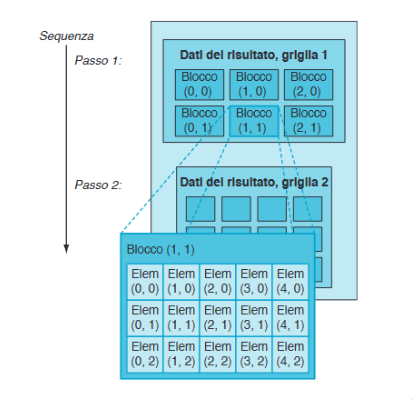
\includegraphics[scale=0.5]{06-GPU/block.png}
    \caption{Scomposizione dei dati in una griglia di blocchi di elementi che vengono calcolati in parallelo.}
\end{figure}

\subsection{Il Paradigma CUDA}

\dfn{CUDA: Programmazione Scalabile e Parallela}{
  CUDA estende i linguaggi C e C++ per sfruttare il parallelismo. Questo fornisce 3 astrazioni fondamentali che permettono una strutturazione chiara del parallelismo: 
  \begin{itemize}
    \item \newfancyglitter{Gerarchia di gruppi}. 
    \item \newfancyglitter{Memorie condivise}. 
    \item \newfancyglitter{Sincronizzazione a barriera}.
  \end{itemize}
}

\nt{Le astrazioni guidano il programmatore a suddividere il problema in spezzoni indipendenti e poi ulteriolmente in spezzoni più piccoli.}

\subsubsection{}

Il programmatore scrive un programma sequenziale che richiame kernel paralleli, i quali possono contenere semplici funzioni o interi programmi. Un kernel viene eseguito in parallelo su un insieme di thread paralleli. Il programmatore organizza questi thread in una gerarchia di blocchi di thread e griglie di blocchi di thread. Un \fancyglitter{blocco di thread} è un insieme di thread concorrenti che possono collaborare tra loro mediante sincronizzazione a barriera e accesso condiviso allo spazio di memoria privato del blocco. Una \fancyglitter{griglia} è un insieme di blocchi di thread concorrenti che possono essere eseguiti ciascuno in modo indipendente, quindi in parallelo. Quando deve essere lanciato in esecuzione un kernel, il programmatore specifica il numero di thread per blocco e il numero di blocchi costituenti la griglia. A ciascun thread viene assegnato un numero identificativo univoco all'interno del blocco di thread che lo contiene, e a ciascun blocco di thread un numero di blocco univoco all'interno della sua griglia.

Il testo di un \fancyglitter{kernel CUDA} è semplicemente una funzione C scritta per un thread sequenziale. È quindi in genere molto semplice da scrivere, soprattutto rispetto al codice parallelo per le operazioni vettoriali. Il parallelismo è determinato in modo chiaro ed esplicito specificando le dimensioni  della griglia di elaborazione e il numero dei suoi blocchi di thread quando il programma kernel viene lanciato in esecuzione. L'esecuzione parallela e la gestione dei thread sono automatiche. 

I thread di un blocco vengono eseguiti in modo concorrente e possono venire sincronizzati in corrispondenza di una \fancyglitter{barriera di sincronizzazione} chiamando la primitiva \textit{syncthreads()}. Questo garantisce che nessun thread del blocco possa proseguire l'esecuzione fino a quando tutti i thread dello stesso blocco non avranno raggiunto la barriera. Dopo averla superata, è garantito che questi thread vedranno i dati che i thread hanno scritto in memoria prima di aver raggiunto la barriera. I thread all'interno di uno stesso blocco, quindi, possono comunicare tra loro scrivendo e leggendo nella memoria condivisa del blocco in corrispondenza della barriera di sincronizzazione. Poiché i thread di un blocco possono condividere la memoria e sincronizzarsi mediante le barriere, essi risiederanno fisicamente nello stesso processore o multiprocessore. Tuttavia, il numero di blocchi di thread può essere significativamente maggiore del numero di processori e fornisce al programmatore totale flessibilità sul grado di granularità che ritiene più conveniente. La virtualizzazione in thread e blocchi di thread permette di scomporre il problema in maniera intuitiva, poiché il numero dei blocchi può essere determinato più dalla dimensione dei dati da elaborare che dal numero di processori del sistema.

Per gestire questa virtualizzazione degli elementi di elaborazione e garantire la scalabilità su più processori, CUDA richiede che i blocchi di thread possano essere eseguiti in modo indipendente: si deve poter eseguire i blocchi in un ordine qualsiasi, in parallelo o in sequenza. Blocchi differenti non hanno possibilità di comunicazione diretta, benché essi possano coordinare le loro attività utilizzando operazioni atomiche di memoria sulla memoria globale visibile da tutti i thread. Questo requisito di indipendenza consente di mandare in esecuzione blocchi di thread in un qualsiasi ordine su un qualsiasi numero di processori rendendo il modello CUDA scalabile su un numero arbitrario di core.

Ogni thread dispone di una \fancyglitter{memoria locale} privata. Ogni blocco dispone di una \fancyglitter{memoria condivisa} visibile a tutti i thread del blocco e tutti i thread hanno anche accesso alla \fancyglitter{memoria globale}.

Cuda ha uno stile molto simile al modello SIMD: il parallelismo è espresso in modo esplicito e ogni kernel viene eseguito con un numero prefissato di thread. Tuttavia, CUDA è più flessibile in quanto il numero di thread e per blocco e griglia varia per ogni kernel.

\begin{figure}[h]
    \centering
    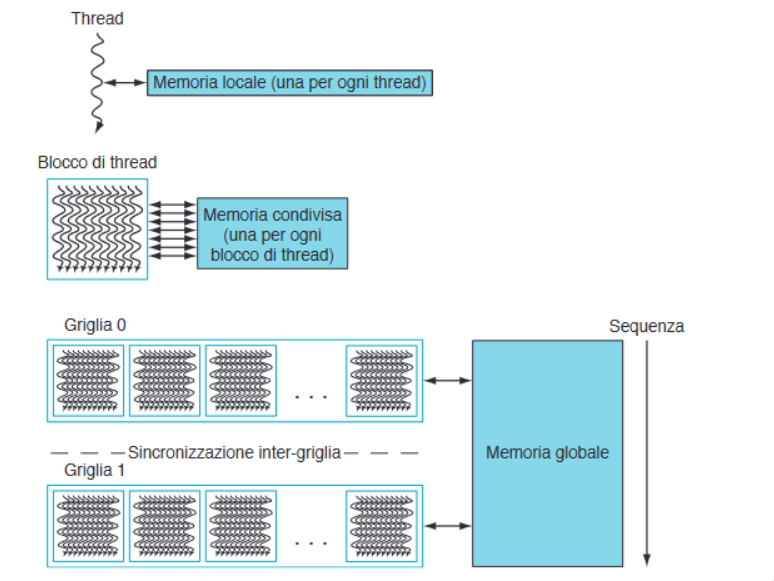
\includegraphics[scale=0.5]{06-GPU/thread.png}
    \caption{I livelli di granularità innestati con le memorie corrispondenti.}
\end{figure}


\section{I Thread}

\subsection{Architettura per il Multithreading}

Le GPU sono multiprocessori composti da multiprocessori, dove ognuno di questi è fortemente multithread. L'alto livello di multithreading è richiesto per vari motivi: 

\begin{itemize}
  \item Nascondere la latenza del caricamento dei dati dalla memoria e della tessitura della RAM. 
  \item Supportare i modelli di programmazione degli shader grafici paralleli a grana fine. 
  \item Supportare i modelli di programmazione per il calcolo parallelo a grana fine. 
  \item Rendere virtuali i processi fisici come thread e blocchi di thread per fornire una scalabilità trasparente. 
  \item Semplificare il modello di programmazione parallela riducendolo alla scrittura di un programma sequenziale per un singolo thread.
\end{itemize}

\subsubsection{}

La latenza del caricamento dei dati e della tessitura della memoria può richiedere centinaia di cicli di clock del processore, poiché le GPU sono tipicamente dotate di cache a flusso continuo di piccole dimensioni. L'organizzazione multithreading aiuta a riempire i tempi di latenza con altre elaborazioni: mentre un thread attende il completamento del caricamento dei dati dalla memoria o del prelievo di una tessitura, il processore può eseguire un altro thread. I modelli di programmazione parallela a grana fine generano migliaia di thread indipendenti, i quali possono mantenere impegnati i processori nonostante le lunghe latenze di memoria viste dal singolo thread. I programmi di grafica e di calcolo istanziano molti thread paralleli rispettivamente per generare immagini complesse e per calcolare matrici di grandi dimensioni che contengono il risultato. 

Per supportare il modello di programmazione ogni thread della GPU dispone dei propri \fancyglitter{registri privati}, di \fancyglitter{memoria privata} dedicata al thread, di un registro \fancyglitter{program counter}  e di un \fancyglitter{registro dello stato di esecuzione del thread}. Proprio per questo è in grado di eseguire un frammento di codice in maniera indipendente. 

Per eseguire in modo efficiente centinaia di thread leggeri e concorrenti, il multiprocessore della GPU implementa il multithreading in hardware, ossia gestisce ed esegue centinaia di thread concorrenti in hardware, senza sovraccarichi per la pianificazione dell'esecuzione.

\subsection{L'Architettura del Multiprocessore}

\begin{figure}[h]
    \centering
    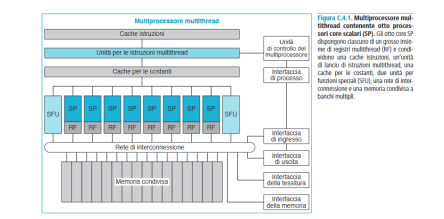
\includegraphics[scale=0.8]{06-GPU/SM.png}
    \caption{SM.}
\end{figure}

L'SM riportato contiene otto SP, ognuno dei quali equipaggiato con tanti registri multithread. 

Ogni core SP contiene unità aritmetiche scalari intere e in virgola mobile che eseguono la maggior parte delle istruzioni. Il processore SP implementa il multithreading in hardware ed è in grado di gestire fino a 64 thread. La pipeline di ogni SP esegue un'istruzione scalare per ogni thread per ogni ciclo di clock, la cui frequenza può variare tra 1.2 GHz e 1.6 GHz, a seconda del modello. Ogni processore SP possiede un insieme di registri (RF) di grosse dimensioni, costituito da 1024 registri a 32 bit di utilizzo generale. Il processore SP può eseguire in modo concorrente molti thread che impiegano pochi registri, oppure un numero minore di thread che necessitano di più registri. 

I programmi CUDA compilati necessitano spesso di 32 registri per thread, limitando così ogni SP a 32 thread e imponendo che un programma kernel abbia al massimo 256 thread per ogni blocco.

\begin{figure}[h]
    \centering
    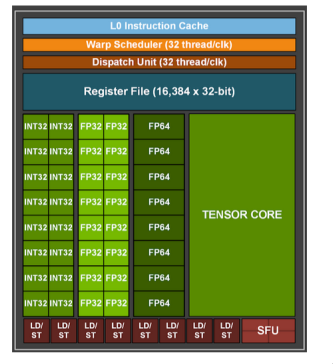
\includegraphics[scale=0.5]{06-GPU/SM-NVIDIA.png}
    \caption{SM di NVIDIA Ampere Architecture.}
\end{figure}

\subsection{SIMT, WARP e WARP Scheduler}

Per gestire ed eseguire in maniera efficiente centinaia di thread che svolgono una grande quantità di programmi diversi, il multiprocessore adotta un'architettura a singola istruzione e thread multipli (\fancyglitter{SIMT}). Essa crea, gestisce pianifica l'esecuzione ed esegue thread concorrenti in gruppi di thread paralleli denominati \fancyglitter{WARP}. Il multiprocessore d'esempio utilizza una dimensione di WARP di  32 thread ed esegue 4 thread in ciascuno degli 8 core SP, in 4 cicli di clock. 

I singoli thread paralleli che compongono un WARP sono dello stesso tipo e partono contemporaneamente dallo stesso indirizzo di codice, ma poi sono liberi di procedere e seguire le biforcazioni del codice in modo indipendente. Ogni volta che viene lanciata in esecuzione un'istruzione, l'unità istruzioni multithread SIMT seleziona un WARP che è pronto per eseguire l'istruzione successiva e invia quell'istruzione ai thread attivi di quel WARP. Un'istruzione SIMT viene diffusa in modo sincrono sui thread paralleli attivi del WARP. 

L'architettura di un processore SIMT è simile a quella dei processori a singola istruzione a corsi di elaborazione multiple di dati. La differenza sta nel fatto che l'architettura SIMT applica un'istruzione a thread multipli indipendenti in parallelo e non semplicemente a corsie multiple di dati. 

Un processore SIMT ottiene piena efficienza e massime prestazioni quando tutti i thread di un WARP seguono lo stesso flusso di esecuzione. Se alcuni thread divergono a causa di un salto condizionato dipendente dai dati, l'esecuzione diventa sequenziale per ognuna delle due diramazioni possibili del codice e, quando tutti i flussi di esecuzione giungono a conclusione, i thread si ricongiungono a un unico flusso. Un codice che contiene una biforcazione del tipo IF ELSE in due flussi di esecuzione di uguale lunghezza ha un'efficienza del 50\%. Per gestire thread indipendenti che divergono e convergono, il multiprocessore utilizza uno stack di sincronizzazione delle diramazioni. WARP differenti vengono eseguiti in maniera indipendente fra loro alla massima velocità possibile, anche se stanno eseguendo flussi di codice comuni o disgiunti. Ne consegue che le GPU SIMT sono decisamente più efficienti e flessibili in relazione ai frammenti di codice divergenti rispetto alle GPU delle precedenti generazioni, poiché i loro WARP sono molto più sottili se paragonati all'ampiezza delle istruzioni SIMD.

Perché il codice sia corretto, il programmatore può sostanzialmente ignorare gli attributi dell'esecuzione SIMT dei WARP ; tuttavia, si può ottenere un incremento sostanziale delle prestazioni avendo cura che il codice raramente abbia bisogno di divergere all'interno di un WARP. 

\noindent
\begin{minipage}[c]{0.6\textwidth} % Larghezza del testo
Un blocco di thread contiene uno o più WARP. L'architettura SIMT condivide l'unità di prelievo e distribuzione delle istruzioni in modo efficiente tra i thread paralleli di uno stesso WARP, ma richiede che tutti i thread del WARP siano attivi per ottenere la massima prestazione. Tale multiprocessore unificato pianifica l'esecuzione ed esegue molteplici tipi di WARP in modo concorrente, permettendo quindi di eseguire WARP di vertice e di pixel. Lo scheduler dei WARP lavora a una frequenza minore di clock del processore, perché deve riempire le corsie di 4 thread per ogni processore core; durante ogni ciclo di pianificazione, esso seleziona un WARP per l'esecuzione di un'istruzione SIMT. Le istruzioni di un WARP vengono lanciate in esecuzione come 4 gruppi di 8 thread, generando i risultati su 4 cicli di clock del processore. Il pianificatore (scheduler) deve selezionare un WARP ogni 4 cicli di clock in modo da lanciare in esecuzione un'istruzione per ciascun ciclo di clock per ogni thread, il che equivale a un IPC = 1,0 per ogni processore core. Dato che i WARP sono indipendenti, le uniche dipendenze possono nascere tra le istruzioni sequenziali di uno stesso WARP. Lo scheduler utilizza una tabella sulla quale annotare le dipendenze tra i registri, per identificare i WARP nei quali i thread attivi sono pronti a eseguire un'istruzione. Questo rende prioritari tutti i WARP pronti e seleziona quindi per il lancio in esecuzione il WARP con la priorità più alta. Il calcolo della priorità deve tener conto del tipo di WARP, del tipo di istruzione, nonché del desiderio di equità nei confronti di tutti i WARP attivi.

\end{minipage}%
\begin{minipage}[c]{0.35\textwidth} % Larghezza dell'immagine
    \centering
    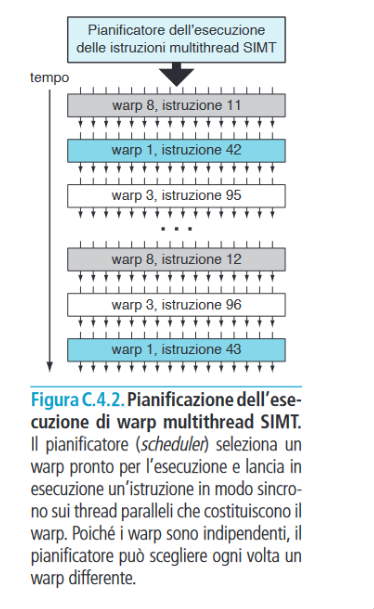
\includegraphics[scale=0.4]{06-GPU/Scheduler_WARP.png}
    \captionof{figure}{Scheduler WARP.}
\end{minipage}

\subsection{Blocchi, Griglie e Sincronizzazione}

L'unità di controllo del multiprocessore e quella delle istruzioni gestiscono i thread e i blocchi di thread. L'unità di controllo accetta richieste di elaborazione e dati in ingresso e arbitra l'accesso alle risorse condivise, comprese l'unità della tessitura, il cammino di accesso alla memoria e i collegamenti di I/O. L'unità di controllo alloca anche un WARP libero e i registri per i thread del WARP e inizia l'esecuzione di WARP sul multiprocessore. Ogni programma dichiara il numero di registri per thread di cui ha bisogno; l'unità di controllo fa partire  un WARP solo quando è in grado di allocare il numero di registri richiesto. Quando tutti i thread di WARP hanno terminato l'esecuzione, l'unità di controllo distribuisce i risultati e libera i registri e le risorse dal WARP.  L'unità di controllo crea \fancyglitter{insiemi di thread cooperativi} (CTA, Cooperative Thread Array), i quali implementano blocchi di thread CUDA sotto forma di uno o più WARP di thread paralleli. Essa crea un CTA quando può produrre tutti i WARP del CTA e allocare tutte le risorse condivise utilizzate dal CTA. L'unità di controllo si accorge quando tutti i thread di un CTA hanno terminato e libera quindi le risorse condivise utilizzate dal CTA e dai suoi WARP. 

La \fancyglitter{sincronizzazione veloce a barriera} permette ai programmi CUDA di comunicare frequentemente attraverso la memoria condivisa e la memoria globale, semplicemente chiamando la funzione \textit{syncthread()} come parte di ogni passo di comunicazione tra thread. Raggruppando i thread in un WARP SIMT di 32 thread si riduce la complessità della sincronizzazione di un fattore 32. I thread attendono a una barriera all'interno dello scheduler dei thread SIMT, in modo da da non utilizzare cicli di processore durante l'attesa. Quando un thread esegue un'istruzione \textit{bar.sync}, incrementa il contatore del numero di thread arrivati alla barriera e lo scheduler registra il thread in attesa. Quando tutti i thread del CTA sono arrivati alla barriera, il conteggio corrisponderà al numero di thread e lo scheduler libererà tutti i thread in attesa, facendo riprendere la loro esecuzione.

\nt{I core LOAD e STORE sono dedicati alla lettura/scrittura sulla memoria globale, sono core dedicati al migliorare l'efficienza delle operazioni riguardanti la memoria.}

\section{Quale codice può girare su una GPU?}

Le GPU sono componenti pensati per l'elaborazione visuale. In generale però, al giorno d'oggi, grazie al paradigma CUDA possono essere utilizzate più facilmente per l'elaborazione di qualsiasi problema che necessiti di un'elevata parallelizzazione durante l'esecuzione. In generale quindi svolgono molto facilmente elaborazioni che, se eseguite sequenzialmente, risulterebbero eccessivamente complesse, mentre non sono ottimali per programmi che di base non permettono la scomposizione del problema in sottoproblemi da parallelizzare. I casi d'uso più emblematici sono:

\begin{itemize}
  \item \fancyglitter{Map} (\fancyglitter{AppyAll}): applica una funzione specificata a ogni elemento di una lista (o di un altro iterabile) e restituisce una nuova lista con i risultati. In pratica trasforma i dati. In altre parole è semplicemente la capacità di applicare una funzione a $n$ item di una lista, dove l'ordine degli item è indifferente.
  \item \fancyglitter{Reduce}: aggrega o combina gli elementi di una lista in un unico risultato utilizzando una funzione binaria specificata (somma, prodotto, etc.). Riduce i dati a un singolo valore. Può essere associativa e commutativa.
\end{itemize}

\nt{Queste due operazioni permettono alle GPU di essere più efficienti nei problemi scomponibili.}

\subsection{Map: VectorAdd}

Nell'ipotesi in cui volessimo creare una semplice funzione che somma due vettori (C = A + B), ci risulta subito chiara la potenza del paradigma MAP. 

\begin{lstlisting}[language=C++, caption={Implementazione sequenziale}]
/**
* Computes the vector addition of A and B into C. The 3 vectors have the same
* number of elements numElements.
*/
void vectorAdd(const float *A, const float *B, float *C, int numElements){
  for (int i = 0; i < numElements; ++i) {
    C[i] = A[i] + B[i] + 0.0f;
  }
}
\end{lstlisting}

\begin{lstlisting}[language=C++, caption={Implementazione CUDA}]
/**
* Computes the vector addition of A and B into C. The 3 vectors have the same
* number of elements numElements.
*/
__global__ void vectorAdd(const float *A, const float *B, float *C, int numElements) {
  int i = blockDim.x * blockIdx.x + threadIdx.x;
  if (i < numElements) {
    C[i] = A[i] + B[i] + 0.0f;
  }
}
\end{lstlisting}

\subsubsection{}

È  evidente che il passaggio da CPU a GPU permetta l'eliminazione del ciclo per effettuare la somma dei vettori. La somma di ogni elemento dei vettori è lasciata a un singolo thread. Solo quando tutti i thread hanno terminato, quindi si ha raggiunto  la barriera di sincronizzazione, si ha raggiunto il risultato.

\subsection{Reduce}

Dato un vettore vogliamo ottenere la somma di tutti i suoi elementi. 

\begin{lstlisting}[language=C++, caption={Implementazione sequenziale}]
/*
 * Parallel sum reduction using shared memory
*/
void reduce(const int *input, int *output, unsigned int n) {
  // Inizializzazione dell'output a zero
  output[0] = 0;

  // Riduzione seriale
  for (unsigned int i = 0; i < n; ++i) {
    output[0] += input[i];
  }
}
\end{lstlisting}

\begin{lstlisting}[language=C++, caption={Implementazione CUDA}]
/*
 * Parallel sum reduction using shared memory
*/
__global__ void reduce(T *g_idata, T *g_odata, unsigned int n) {
  // Handle to thread block group
  cg::thread_block cta = cg::this_thread_block();
  T *sdata = SharedMemory<T>();

  // load shared mem
  unsigned int tid = threadIdx.x;
  unsigned int i = blockIdx.x * blockDim.x + threadIdx.x;

  // uso la shared memory come una cache programmata della global memory
  sdata[tid] = (i < n) ? g_idata[i] : 0;

  //barriera di sincronizzazione, aspetto che tutti i thread arrivino a questo punto.
  cg::sync(cta);

  // do reduction in shared mem
  for (unsigned int s = 1; s < blockDim.x; s *= 2) {
    // modulo arithmetic is slow!
    if ((tid % (2 * s)) == 0) {
      sdata[tid] += sdata[tid + s];
    }
    cg::sync(cta);
  }

  // write result for this block to global mem
  if (tid == 0) g_odata[blockIdx.x] = sdata[0];
}
\end{lstlisting}

\subsubsection{}

A questo punto sono chiare due cose: 

\begin{enumerate}
  \item Il codice scritto per una GPU risulta più corposo e di difficile interpretazione, inoltre è il programmatore a doverlo rendere efficiente e controllare lo stato di esecuzione (shared memory e barriera di sincronizzazione). 
  \item Si ha un aumento notevole di prestazioni da O($n$) a O(log $n$) per lo stesso problema.
\end{enumerate}

\subsection{Copiare da Global Memory a Shared Memory}

Per copiare da global a shared memory si assegna una variabile che è in shared memory a una che è in global memory. Per esempio nella reduce: 

\begin{lstlisting}[language=C++]
  sdata[tid] = (i < n) ? g_idata[i] : 0;
\end{lstlisting}

\nt{Copiare le variabili in shared memory è utile in quanto la shared memory è molto più veloce (1 ciclo per accedervi rispetto ai +400 cicli per accedere alla global memory). Importarsi in questo modo le variabili è come se si andasse a creare una \fancyglitter{cache programmabile}, in cui decide il programmatore cosa avvicinare.}




